\subsubsection{Sleep modes}
The comparison of the three different sleep modes is based on the above described setup.
Table \ref{tab:sleep_modes_15min} shows the measured energy consumption in Coulomb which is equal to $As$.
The average power consumption in $mA$ is also listed.

\begin{table}[htbp]
\caption{Measured sleep power consumption}
\begin{center}
\begin{tabular}{|c|c|c|}
\hline
\textbf{Sleep mode}&\textbf{Used energy $[As]$}&\textbf{Average current $[mA]$}\\
\hline
\textbf{Modem sleep} & 323.77As & 36.9mA\\
\textbf{Light sleep} & 182.31As & 20.46mA\\
\textbf{Deep sleep}  & 1.12As   & 0.127mA\\
\hline
\end{tabular}
\label{tab:sleep_modes_15min}
\end{center}
\end{table}

By using the light sleep mode instead of the modem sleep mode, we were able to reduce the energy consumption by a factor of $\approx 1.7$.
In addition, by using the deep sleep, we managed to reduce the energy consumption by a factor of $\approx 290$.
These results clearly show the huge advantage of the deep sleep mode compared to the default enabled modem sleep mode.
The Fig. \ref{fig:sleep_compare_boxplot} illustrates in which range the power consumption is most often in the different modes.

\begin{figure}[H]
    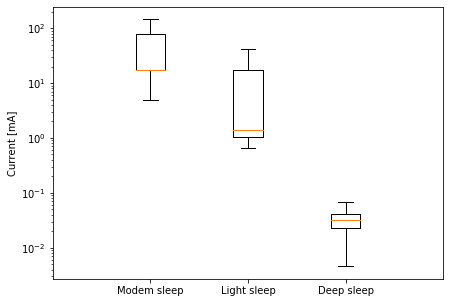
\includegraphics[width = \linewidth]{fig/sleep_compare_boxplot.png}
    \caption{Box plot to illustrate in which rage the power consumption is most often. Y-Axis has a logarithmic scale.}
    \label{fig:sleep_compare_boxplot}
\end{figure}